\usetikzlibrary{positioning}
\usetikzlibrary{calc}
\usetikzlibrary{babel}
\definecolor{pastelred}{HTML}{D37676}
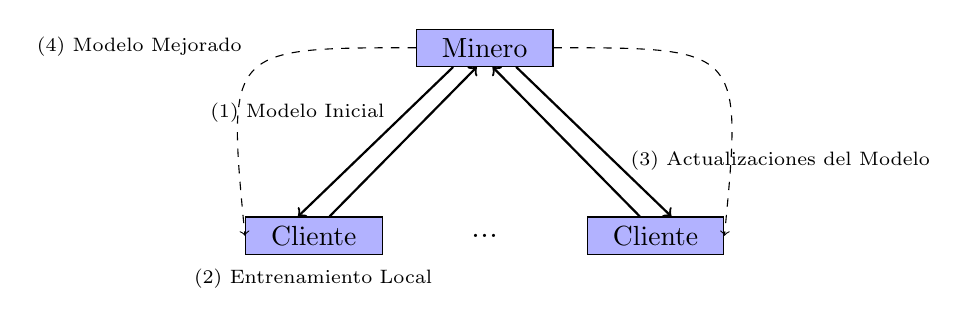
\begin{tikzpicture}[
scale=2,
clientnode/.style={rectangle, draw=black!100, text width=1.5cm,
align=center, anchor=center, fill=blue!30},
textnode/.style={}
]

%Nodes
\node[clientnode] (miner) {Minero};
\node[textnode] (dots) [below=2cm of miner] {\large ...};
\node[clientnode] (client1) [left=of dots] {Cliente};
\node[clientnode] (client2) [right=of dots] {Cliente};
\node[textnode] (label1) [below=0.05cm of client1] {\textsuperscript{(2) Entrenamiento Local}};
\node[textnode] (label2) [left=0.05cm of client2] {};

%Coordinates
\coordinate (miner1) at ($ (miner.south) - (0.2,0) $);
\coordinate (miner2) at ($ (miner.south) - (0.05,0) $);
\coordinate (miner3) at ($ (miner.south) + (0.05,0) $);
\coordinate (miner4) at ($ (miner.south) + (0.2,0) $);
\coordinate (client11) at ( $ (client1.north) - (0.1, 0) $ );
\coordinate (client12) at ( $ (client1.north) + (0.1, 0) $ );
\coordinate (client21) at ( $ (client2.north) - (0.1, 0) $ );
\coordinate (client22) at ( $ (client2.north) + (0.1, 0) $ );

%Lines
\draw[thick, ->] (miner1) -- (client11) node[midway, above left] {};
\draw[thick, ->] (miner4) -- (client22) node[midway, above right] {};
\draw[thick, ->] (client12) -- (miner2) node[midway, below right] {};
\draw[thick, ->] (client21) -- (miner3) node[midway, below left] {};

\draw[dashed, ->] (miner.west) .. controls +(left:1.2cm) .. (client1.west) node[midway, above left] {\textsuperscript{(4) Modelo Mejorado}};
\draw[dashed, ->] (miner.east) .. controls +(right:1.2cm) .. (client2.east) node[midway, above right] {};


\node[textnode, above=1cm of client11] {\textsuperscript{(1) Modelo Inicial}};
\node[textnode, above right=0.4cm and 3.7cm of client12] {\textsuperscript{(3) Actualizaciones del Modelo}};
    
\end{tikzpicture}